
\documentclass[18pt]{beamer}

\geometry{paperwidth=128mm,paperheight=096mm}

\usepackage{templates/beamerthemekit}
%\usepackage{templates/beamerthemekitwide}

%% TITLE PICTURE
\titleimage{KIT-Titel}

%% TITLE LOGO
\titlelogo{kitlogo}

% for python listings
\usepackage{minted}
\newminted{python}{gobble=4,fontsize=\scriptsize}
\newminted{bash}{gobble=4,fontsize=\scriptsize}
\newmintinline{python}{fontsize=\scriptsize}
\newmintinline{bash}{fontsize=\scriptsize}

% for underlining
\usepackage[normalem]{ulem}

% for urls
\usepackage{hyperref}

% for interface scheme
\usepackage{tikz}
\usetikzlibrary{positioning}
\usetikzlibrary{decorations.text}
\usetikzlibrary{decorations.pathmorphing}
\usetikzlibrary{fit}
\usetikzlibrary{shapes}





\title[PIRS: current possibilites]{Python Interfaces for Reactor Simulations:\\ Concept, ways to use, examples}
\subtitle{INR Seminar "Nukleare Energieerzeugung"}
\author{Anton Travleev}

\institute{Institute for Neutron Physics and Reactor Technology}

% extra-slides for begin of section
\AtBeginSection[]
{
    \begin{frame}
    \frametitle{Outline}
    \tableofcontents[currentsection, 
                     hideothersubsections,
                     sectionstyle=show/hide,
                     subsectionstyle=show/hide,]
    \end{frame}
}

% the presentation starts here
\begin{document}

% change the following line to "ngerman" for German style date and logos
\selectlanguage{english}

%title page
\begin{frame}
\titlepage
\end{frame}

%table of contents
\begin{frame}{Outline}
\tableofcontents
\end{frame}


\section{Introduction to PIRS}
\subsection{What it is}
% Definition with explanation
\begin{frame}\frametitle{What is PIRS}

    \begin{block}{PIRS: Python Interfaces for Reactor Simulations}

        A package for \uline{Python} programming language, to facilitate
        \uline{interaction} with reactor calculation codes.
    \end{block}

    \begin{columns}
        \column{0.45\textwidth}

        \pause
        \begin{block}{Python}
        \begin{itemize}

            \item www.python.org

            \item Free 

            \item Interpreted: cross-platform but slow

            \item Big community: lot of ready-to-use solutions


        \end{itemize}
        \end{block}

        \column{0.45\textwidth}

        \pause
        \begin{block}{Interaction with code}
        \begin{itemize}
            
            \item Model description

            \item Generation of Input file(s)

            \item Job submission

            \item Reading of calculation results

        \end{itemize}
        \end{block}
    \end{columns}
\end{frame}

% History: why Python, task behind: coupling MCNP and SCF, build principles (light-weight, general tool, modular)
\begin{frame}\frametitle{Background}
    \begin{block}{Prerequisites}
    \begin{itemize}
        \item Author's Experience with Python and MCNP 
        \item HPMC project: goal to couple Monte-Carlo with TH for PWR-like geometries from pin to reactor core
        \item Previous coupling schemes -- mix of programming languages (from shell to fortran), higly specific to geometry
    \end{itemize}
    \end{block}

    \begin{block}{Idea}
    \begin{itemize}
        \item Light-weight: e.g. to deploy on cluster's local account
        \item General tool: geometry-independent, not only for coupled calculations
        \item Everything should be specified in terms of a programming language
    \end{itemize}
    \end{block}
\end{frame}

\begin{frame}\frametitle{PIRS concept}
    % when implementing coupled calcs from scratch, one needs to define things that can be put into several types:
    %    * data common to all codes, i.e. geometry description of calculational model, meshes to represent dependent variables
    %    * code-specific data like material composition or T/H properties
    %    * organization of data flow

    \begin{itemize}
        \item Geometry definition: should be reusable in all codes, defined in terms, independent on any particular code.

        \item Convenien way to handle distribution of dependent variables (heat deposition, temperature and material density axial distributions)

        \item Interface consists of two parts:
            \begin{itemize}
                \item Low-level interface: "knows" syntax of input file(s), can read output files, can start code and wait until it completes
                \item High-level interface: converts code-independent geometry together with additionally specified code-specific data to low-level interfaces, and puts results of
                      calculations back to code-independent geometry.
            \end{itemize}
    \end{itemize}
\end{frame}


\subsection{Concept}
% Interface concept: show the scheme, explain data flow, explain what user and developers use.
\begin{frame}[fragile]
    \frametitle{PIRS concept scheme}
    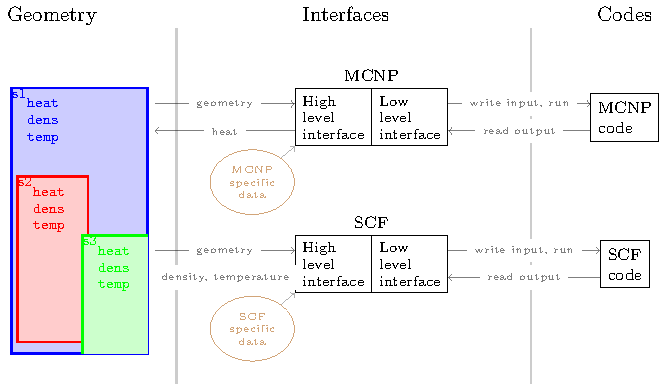
\includegraphics[width=\textwidth]{scheme_wrapper.pdf}
\end{frame}



\subsection{Content}
% Package content: list of subpackages, only general overview
\begin{frame}[fragile]
    \frametitle{PIRS classes and functions}

    \begin{block}{Geometry construction}
    \begin{columns}
        \column{0.6\textwidth}
        \begin{pythoncode}
            from pirs.solids import Cylinder, Box
            from pirs.solids import zmesh
        \end{pythoncode}
        \column{0.4\textwidth}{\scriptsize

        Classes to represent solids -- basic elements to describe geometry and axial meshes for dependent variables.

        }
    \end{columns}
    \end{block}

    \begin{block}{High-level interfaces}
        \begin{pythoncode}
            from pirs import McnpInterface
            from pirs import ScfInterface
        \end{pythoncode}
    \end{block}
\end{frame}


\begin{frame}[fragile]
    \frametitle{PIRS classes and functions}

    \begin{block}{Low-level interface to MCNP}
    \begin{columns}
        \column{0.8\textwidth}
        \begin{pythoncode}
        from pirs.mcnp import Material, MaterialCollection
        from pirs.mcnp import MeshTally, TallyCollection
        from pirs.mcnp import Xsdir
        from pirs.mcnp import Surface, Volume, SurfaceCollection
        from pirs.mcnp import Cell, Model
        \end{pythoncode}
        \column{0.2\textwidth}{\tiny

        Classes to represent data for MCNP input file: mateirals, tallies, surfaces, cells, etc.

        }
    \end{columns}
    \end{block}

    \begin{block}{Low-level interface to SCF}
    \begin{columns}
        \column{0.8\textwidth}
        \begin{pythoncode}
        from pirs.scf2 import Input, RodMaterial
        from pirs.scf2.variables import ScfVariable, ScfTable
        from pirs.scf2 import read_output, OutputTable
        \end{pythoncode}
        \column{0.2\textwidth}{\tiny

        Classes to represent data for SCF input file: variables, tables, switches, etc.

        }
    \end{columns}
    \end{block}
\end{frame}


\begin{frame}[fragile]
    \frametitle{PIRS classes and functions}

    \begin{block}{Tools}
    \begin{columns}
        \column{0.7\textwidth}
        \begin{pythoncode}
        from pirs.tools import LoadMap
        from pirs.tools import load, dump
        from pirs.tools.plots import MeshPlotter, colormap
        \end{pythoncode}
        \column{0.3\textwidth}{\tiny
        Pseudo-graphics definition of core loading maps, functions to dump
        current calculational state to hard drive and to read it; functions to
        plot geometry and distribution of variables.

        }
    \end{columns}
    \end{block}

    \begin{block}{Base classes}
    \begin{columns}
        \column{0.8\textwidth}
        \begin{pythoncode}
        from pirs.core.tramat import Nuclide, Mixture, zai
        from pirs.core.trageom import Vector3, pi, pi2
        from pirs.core.scheduler import Job, Scheduler
        from pirs.core.scheduler enva, WorkPlace, InputFile
        \end{pythoncode}
        \column{0.2\textwidth}{\tiny
        Parent classes used in PIRS in several places. Not needed to end-user.

        }
    \end{columns}
    \end{block}

\end{frame}



\section{PIRS installation and setup}
% dependencies
% user-local installation, e.g. for use on a server
% environment variables
\begin{frame}[fragile]
    \frametitle{Dependencies}
    \begin{block}{Python interpreter}
    \begin{itemize}
        \item PIRS is developed with Python 2.7 and tested with Python 2.6.
        \item Python 3.x: ?
        \item Linux distributions usually have Python 2.6 or 2.7 preinstalled. Under Windows, administrator rights are necessary to install Python.
    \end{itemize}
    \end{block}

    \begin{block}{Optional third-party packages}
    \begin{itemize}

        \item uncertainties package, http://pythonhosted.org/uncertainties/. To handle results of 
    Monte-Carlo calculations.

        \item Matplotlib package, http://matplotlib.org/. To generate geometry and result plots.
    \end{itemize}
    \end{block}
\end{frame}

\begin{frame}[fragile]
    \frametitle{PIRS setup}
    \begin{block}{Install package}
        \begin{bashcode}
            $> tar -xzf pirs-X.Y.Z.tar.gz
            $> cd pirs-X.Y.Z
            $> python setup.py install --user
        \end{bashcode}

        The \bashinline/--user/ option to install locally
    \end{block}

    \begin{block}{Define environmental variables}
        \begin{bashcode}
            $> export DATAPATH=/path/to/folder/with/xsdir
            $> export MCNP=/path/to/mcnp/executable
            $> export SCF=/path/to/scf/executable
        \end{bashcode}

        \begin{itemize}
            \item \bashinline/$DATAPATH/: Path to default xsdir used to define available cross-sections.

            \item \bashinline/$MCNP/ and \bashinline/$SCF/: paths to code executables.
        \end{itemize}

    \end{block}
\end{frame}


\section{Examples}

\subsection{MCNP interface minimal example: K-inf in nat. U}
\begin{frame}[fragile]
    \frametitle{K-inf in nat. U}

    \begin{columns}
        \column{0.7\textwidth}
        \inputminted[frame=single,fontfamily=tt,fontsize=\scriptsize]{python}{examples/ex1.py}

        \column{0.3\textwidth}{\tiny
        \begin{itemize}
            \item Default box dimensions 1x1x1 cm
            \item \pythoninline/b.dens/ represents density axial distribution. 
            \item general model contain material names, which meaning/properties are specified in the
                  code interface.
            \item \pythoninline/McnpInterface/ -- MCNP high-level interface.
            \item \pythoninline/Material/ -- part of low-level interface.
        \end{itemize}
        }
     \end{columns}
\end{frame}

\begin{frame}[fragile]
    \frametitle{Output}
    \inputminted[frame=single,fontfamily=tt,fontsize=\scriptsize]{python}{examples/ex1.out}
\end{frame}

\begin{frame}[fragile]
    \frametitle{MCNP input file}
    \begin{columns}
        \column{0.7\textwidth}
        \inputminted[frame=single,fontfamily=tt,fontsize=\scriptsize]{bash}{examples/mcnp0/i_}
        \column{0.3\textwidth}{\tiny
        \begin{itemize}
            \item Cell, surface and material numbers assigned automatically
            \item Macrobodies are used when possible
            \item Cross-section suffix chosen for default temperature from existing xs in xsdir
        \end{itemize}
        }
    \end{columns}
\end{frame}




\subsection{Geomety example: single pin}
\begin{frame}[fragile]
    \frametitle{Geometry of single pin cell}

    \begin{columns}
        \column{0.6\textwidth}
        \inputminted[frame=single,fontfamily=tt,fontsize=\tiny]{python}{examples/ex2_geom.py}

        \column{0.4\textwidth}{\scriptsize
        \begin{itemize}
            \item Solid's dimensions can be specified using correspondent attributes    
            \item Solid can be inserted into another
            \item Solid can be positioned with respect to its container
            \item \pythoninline/colormap/ function uses Matplotlib
        \end{itemize}
        }
     \end{columns}
\end{frame}

\begin{frame}[fragile]
    \frametitle{Plots}
    \begin{columns}
        \column{0.5\textwidth}
            {\tiny z plane}
            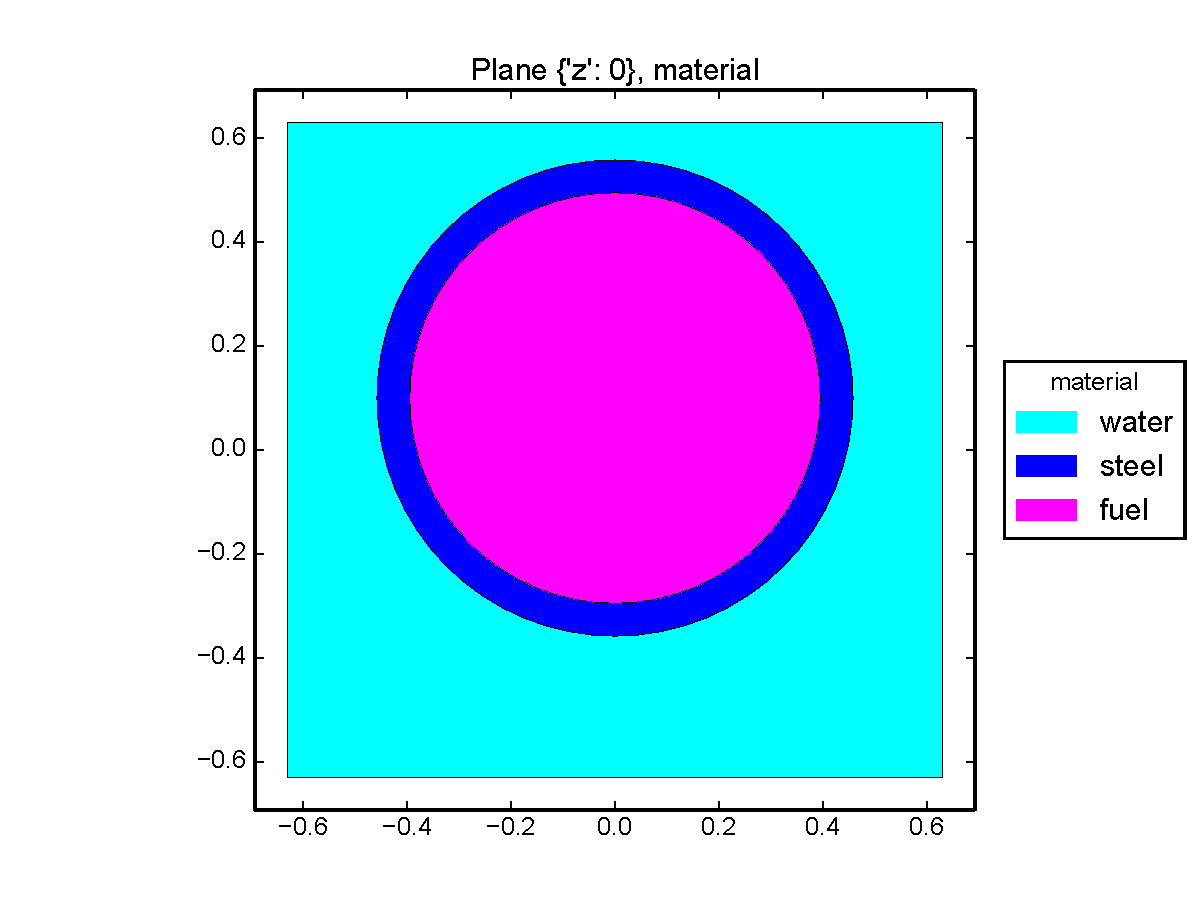
\includegraphics[width=\textwidth]{examples/ex2z.pdf}
        \column{0.5\textwidth}
            {\tiny x plane}
            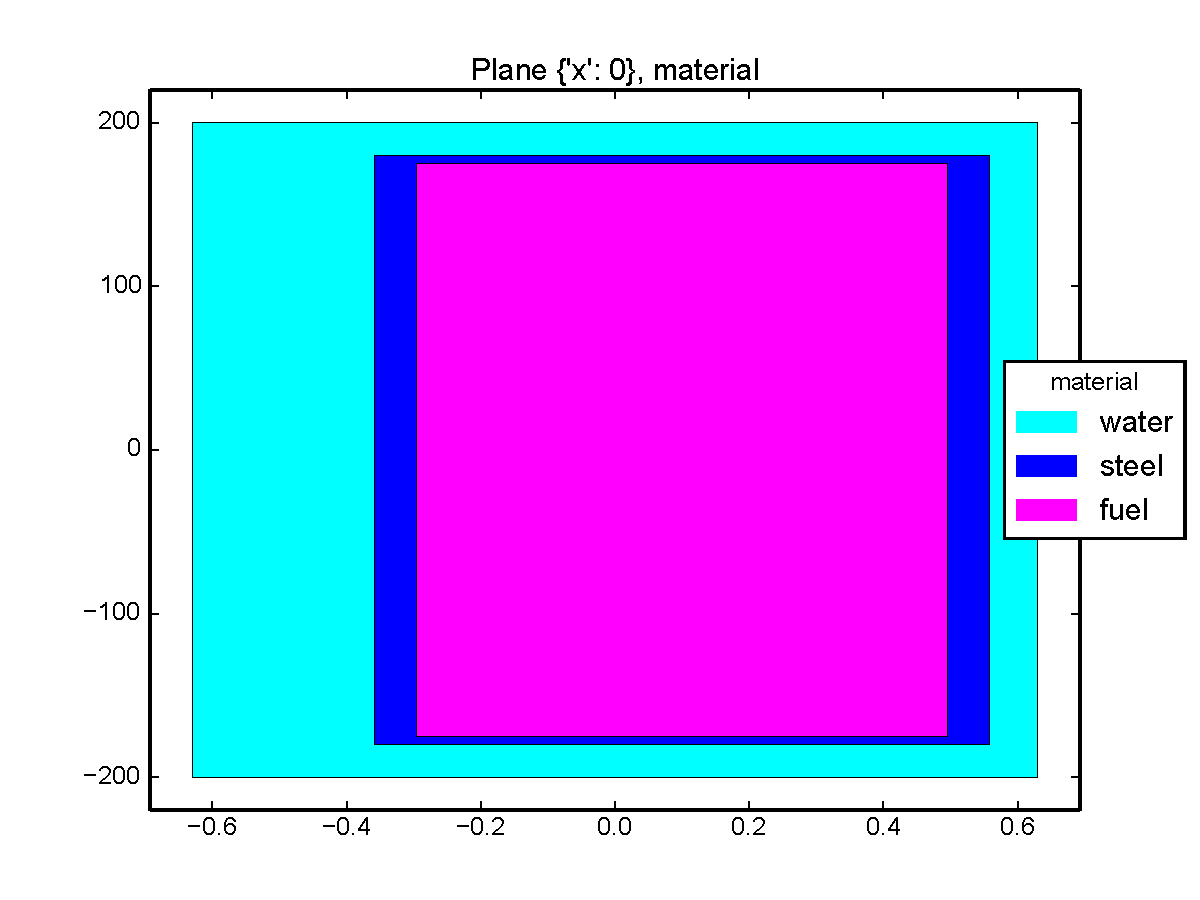
\includegraphics[width=\textwidth]{examples/ex2x.pdf}
    \end{columns}
\end{frame}

\subsection{Axial distributions}
\begin{frame}[fragile]
    \frametitle{Axial distributions}

    \begin{columns}
        \column{0.6\textwidth}
        \inputminted[frame=single,fontfamily=tt,fontsize=\tiny]{python}{examples/ex2_vars.py}

        \column{0.4\textwidth}{\scriptsize
        \begin{itemize}
            \item \pythoninline/get_child()/ method refers to one of the solids used in geometry definition. 
            \item each solid has \pythoninline/temp/, \pythoninline/dens/ and \pythoninline/heat/ attributes
                  to represent axial profiles of temperature, density and heat, respectively.
            \item \pythoninline/set_grid()/ method sets amount and relative thickness of axial mesh layers; first list element corresponds lower layer.

            \item \pythoninline/colormap()/ can generate colormaps of axial profiles.
        \end{itemize}
        }
     \end{columns}
\end{frame}

\begin{frame}[fragile]
    \frametitle{Plots}
    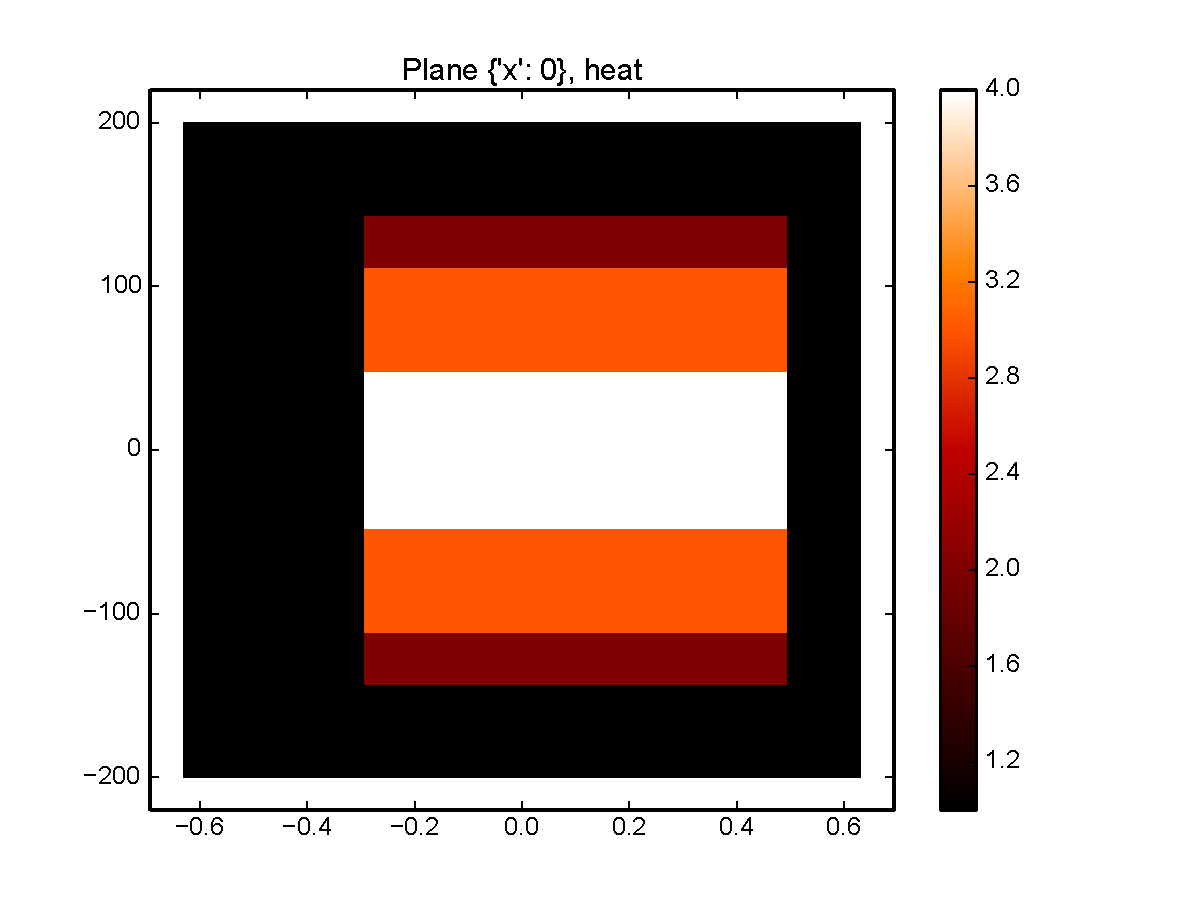
\includegraphics[width=0.5\textwidth]{examples/ex2t.pdf}
\end{frame}

\subsection{Coupled calculations}
\begin{frame}[fragile]
    \frametitle{Coupled calculations}

    \begin{columns}
        \column{0.6\textwidth}
        \inputminted[frame=single,fontfamily=tt,fontsize=\tiny]{python}{examples/ne4_coupl.py}

        \column{0.4\textwidth}{\scriptsize
        \begin{itemize}
            \item given geometry \pythoninline/a/ and code-specific data in \pythoninline/MI/ and \pythoninline/SI/ were already defined
            \item \pythoninline/run()/ method generates input, starts code, waits until it completes, reads results and returns copy of \pythoninline/a/ that contain in \pythoninline/heat/ attributes MCNP results.
        \end{itemize}
        }
     \end{columns}
\end{frame}


\subsection{Square lattices}
\begin{frame}[fragile]
    \frametitle{Square lattices}

    \begin{columns}
        \column{0.6\textwidth}
        \inputminted[frame=single,fontfamily=tt,fontsize=\tiny]{python}{examples/ex3_lat.py}

        \column{0.4\textwidth}{\scriptsize
        \begin{itemize}
            \item \pythoninline/grid/ attribute describes superimposed rectangular lattice, which can be used to
                position inserted solids.
            \item \pythoninline/grid.insert()/ method is similar to \pythoninline/insert()/ method, but inserted solid
                is placed in lattice element specified as 1-st agrument.
            \item \pythoninline/copy_tree()/ method returns deep copy of a solid (i.e. all inserted solids are copied as well)
            \item \pythoninline/grid.center()/ method positions lattice with respect to solid in a way that rectangle circumscribing all
                solids inserted into lattice elements, is centered.
        \end{itemize}
        }
     \end{columns}
\end{frame}

\begin{frame}[fragile]
    \frametitle{Plots}
    \begin{columns}
        \column{0.5\textwidth}
        {\tiny Lattice not centered: (0,0,0)-th element is at origin}
            \includegraphics[width=\textwidth]{examples/ex3_1.pdf}
        \column{0.5\textwidth}
        {\tiny After \pythoninline/grid.center()/ method}
            \includegraphics[width=\textwidth]{examples/ex3_2.pdf}
    \end{columns}
\end{frame}
% 
% 
% 
% 
\begin{frame}[fragile]
    \frametitle{Features of  high-level interfaces}
    \begin{itemize}
        \item Complex geometries can be defined with operations of insertion and translation with respect to container.

        \item MCNP high-level interface can handle any geometry (theoretically).
            \begin{itemize}
                \item \pythoninline/grid/ is modelled with lattices in MCNP input file
                \item solids are compared: equal solids represented using the same universe
                \item If possible, macrobodies are used
                \item non-trivial heat axial distributions considered as definition of heat deposition meshtally
                \item temperature axial meshes define \bashinline/tmp/ cell options and are used to find xs data. 
            \end{itemize}

        \item SCF high-level interface  is limited: 
            \begin{itemize}
                \item only square bundles of heated rods or unheated cylinder channels
                \item all solids in model must have same height
                \item coolant-centerd sub-channels are modelled in SCF, but
                \item rod-centered temperatures and densities are returned back to model
            \end{itemize}
    \end{itemize}
\end{frame}

\subsection{Material nuclide composition}
\begin{frame}[fragile]
    \frametitle{Compound materials}
    \begin{columns}
        \column{0.45\textwidth}
        \inputminted[frame=single,fontfamily=tt,fontsize=\scriptsize]{python}{examples/ex2_mat.py}
        \column{0.55\textwidth}{\scriptsize
        \begin{itemize}
            \item Materials can be multiplied by scalar and added 
            \item \pythoninline/thermal/ attribute specifies part of thermal data name. Particular table is chosen to fit temperature.
            \item \pythoninline/sdict/ dictionary specifies substitutions if cross-sections not available. 
            \item \pythoninline/card/ method returns multi-line string containg definition of material for MCNP input file. Can be used separately.
            \item Generally, \pythoninline/Material/ class constructor takes a list of tuples of the form \pythoninline/(spec, amount, unit)/, where
                \pythoninline/spec/ -- string, integer or Material instance, \pythoninline/amount/ -- amount of ingredient and \pythoninline/unit/ --flag specifying units.
        \end{itemize}
        }
     \end{columns}
\end{frame}
\begin{frame}[fragile]
    \frametitle{Compound materials, output}
    \begin{columns}
        \column{0.7\textwidth}
        \inputminted[frame=single,fontfamily=tt,fontsize=\tiny]{bash}{examples/ex2_mat.out}
        \column{0.3\textwidth}{\tiny
        \begin{itemize}
            \item Material \pythoninline/w/ contains nuclide O-18, but in MCNP material card it is substituted with O-16.
            \item Material card is formatting string, thus actual material numbers is simple to insert.
            \item Thremal data are chosen among cross-sections containing 'lwtr' in its name with closest temperature.
        \end{itemize}
        }
     \end{columns}
\end{frame}


\begin{frame}[fragile]
    \frametitle{Implicit material definition}
    {\scriptsize 
    Problem: Given U and Pu isotopic vectors in \% by weight, define MOX having
    10\% at. of fissile nuclides.
    }
    \begin{columns}
        \column{0.6\textwidth}
        \inputminted[frame=single,fontfamily=tt,fontsize=\tiny]{python}{examples/ex_mox.py}
        \column{0.4\textwidth}{\scriptsize
        \begin{itemize}
            \item U and Pu elements, \pythoninline/u/ and \pythoninline/p/, are defined using grams.
            \item Initially, \pythoninline/mox/ is defined using equal amounts (moles) of U and Pu oxide.
            \item Objective function \pythoninline/of()/ takes a material instance as argument and returns deviation of ratio of 
                fissile nuclides to all heavy metal nucled from 5\% 
            \item Method \pythoninline/tune()/ changes amount of specified ingredients until objective function returns (almost) zero.
        \end{itemize}
        }
     \end{columns}
\end{frame}
\begin{frame}[fragile]
    \frametitle{Implicit material definition, output}
    \begin{columns}
        \column{0.7\textwidth}
        \inputminted[frame=single,fontfamily=tt,fontsize=\tiny]{bash}{examples/ex_mox.out}
        \column{0.3\textwidth}{\scriptsize
        After \pythoninline/tune()/ method, amount of fissile nuclides is 0.0347 mol and amount of all heavy metal nuclides is 0.347 mol in
        definition of \pythoninline/mox/ material.
        }
     \end{columns}
\end{frame}



\section{Results of coupled calculations}

\subsection{Model}
\begin{frame}[fragile]
    \frametitle{3x3 minicore}
    \begin{itemize}
        \item Based on NEA PWR transient benchmark
        \item 6 UOX and 3 MOX 17x17 assemblies, 20 axial layers
        \item UOX has 2 types of rods: fuel pins and water channels
        \item MOX has 5 types of rods: 3 fuel pins, water channels and WABA
        \item Can be represented as single bundle with 51x51 rods
        \item To show performance of codes, provide benchmark for comparison
    \end{itemize}
    \begin{columns}
        \column{0.33\textwidth}
        \includegraphics[width=\textwidth]{examples/a_model_z.pdf}
        \column{0.33\textwidth}
        \includegraphics[width=\textwidth]{examples/a_model_zu.pdf}
        \column{0.33\textwidth}
        \includegraphics[width=\textwidth]{examples/a_model_zm.pdf}
    \end{columns}

\end{frame}


\subsection{Calculations}
\begin{frame}[fragile]
    \frametitle{Calculations}
    \begin{itemize}
        \item IC2 cluster, 1 node with 16 cores
        \item Standard meshtally to compute heat deposition

            \begin{bashcode}
        Iteration        kcode                 wall time    Num of cells            
                0       500000  1.0  30  100     0:05:27            3544 
                1       809016  1.0  30  100     1:38:43          107634
                2      1096763  1.0  30  100     1:52:51          107634
                3      1374895  1.0  30  100     2:06:26             ...  
                4      1647439  1.0  30  100     2:19:16          
                5      1916300  1.0  30  100     2:29:45             ... 

               20      5549120  1.0  30  100     5:05:40             ...
               21      5804749  1.0  30  100     5:15:52 
               22      6060130  1.0  30  100     5:27:00 
               23      6315284  1.0  30  100     5:38:33 
               24      6570230  1.0  30  100     5:49:10 
               25      6824985  1.0  30  100     6:00:09             ...
               26      7079562  1.0  30  100     6:12:28          107634

            \end{bashcode}
        \item MCNP initialization time 15 -- 50 min

    \end{itemize}
\end{frame}

\subsection{Results}

\begin{frame}[fragile]
    \frametitle{Heat deposition}
    \includegraphics[width=\textwidth]{examples/map_anton_e26_k01k08k19_Power.pdf}

    \includegraphics[width=\textwidth]{examples/map_anton_e26_i09i26j09j26j43_Power.pdf}
\end{frame}

\begin{frame}[fragile]
    \frametitle{Fuel temperature}
    \includegraphics[width=\textwidth]{examples/map_anton_e26_k01k08k19_Tfuel.pdf}

    \includegraphics[width=\textwidth]{examples/map_anton_e26_i09i26j09j26j43_Tfuel.pdf}
\end{frame}

\begin{frame}[fragile]
    \frametitle{Comparison with other calculations}

    \begin{itemize}
        \item Solution 1: Internal MCNP-SCF coupling (A. Ivanov, INR)
        \item Solution 2: PIRS-based 
        \item Solution 3: Internal Serpent2-SCF coupling (M. Daeubler, INR)
        \item Solution 4: Internal MCNP-SCF coupling (E. Hoogenboom, DNC)
    \end{itemize}

\end{frame}

\begin{frame}[fragile]
    \frametitle{K-eff and statistics}
    \begin{columns}
        \column{0.6\textwidth}
        \includegraphics[width=\textwidth,page=22,trim=0.8in 4.0in 1.0in 1.6in,clip=true]{examples/benchmark_.pdf}
        \column{0.4\textwidth}{\scriptsize
        \begin{itemize}
            \item Difference in K-eff about 200 pcm (except solution 4 with lower statistics)
            \item Different relaxation schemes
            \item Fuel temperature converged to less than 0.2\%
        \end{itemize}
        }
    \end{columns}
\end{frame}

\begin{frame}[fragile]
    \frametitle{Heat deposition}
    \begin{columns}
        \column{0.6\textwidth}
        \includegraphics[width=\textwidth,page=25,trim=1.2in 2.6in 0.65in 5.6in,clip=true]{examples/benchmark_.pdf}
        \column{0.4\textwidth}{\scriptsize
        \begin{itemize}
            \item Shift to lower part: coolant density (slowing down and leakage) and fuel temperature (U8 capture).
            \item Solution 4 has the strongest power, Tf and density axial shift.
            \item Tf axial shift more pronounced in S2, while density axial
                shift -- in S3. Since power shift is stronger in S2,  Tf has
                larger impact onto power axial profile in comparison to
                density.
        \end{itemize}
        }
    \end{columns}
\end{frame}

\begin{frame}[fragile]
    \frametitle{Fuel temperature}
    \begin{columns}
        \column{0.7\textwidth}
        \includegraphics[width=\textwidth,page=25,trim=1.2in 6.6in 0.65in 1.6in,clip=true]{examples/benchmark_.pdf}
        \column{0.3\textwidth}{\scriptsize
        \begin{itemize}
            \item Average values within 0.3 K (1. K for s.4)
            \item Max. values within 20 K
            \item Tfuel shifted to lower part
            \item U assemblies are about 50 K hotter. Difference grows from solution 1 to 4.
        \end{itemize}
        }
    \end{columns}
\end{frame}

\begin{frame}[fragile]
    \frametitle{Solution-to-solution max. differences}
    \begin{columns}
        \column{0.6\textwidth}
        \includegraphics[width=\textwidth,page=27,trim=1.2in 2.2in 0.65in 5.8in,clip=true]{examples/benchmark_.pdf}
        \column{0.4\textwidth}{\scriptsize
        \begin{itemize}
            \item Max. difference in Tf and coolant density found between solutions 1 and 3: 26 K and 1.66 kg/m3.
            \item Colormaps for differences (not shown) demonstrate that they are systematic.
            \item Discrepancies in results still need analysis, but 
                  overall good agreement indicate that all implementations are free from coding errors.
        \end{itemize}
        }
    \end{columns}
\end{frame}




% History: as a benchmark for several different coupling implementations
% Description of model: criteria: show complexity, close to existing benchmark
% calculation statistics
% results


\section{Outlook}
% Availability of PIRS: in INR, and outside KIT.
% Ongoing work: interface to SERPENT
% Making it open source.

\begin{frame}[fragile]
    \frametitle{Ongoing work}

    \begin{itemize}
        \item Interface to Serpent-2 using multi-physics interface. Toward full-core coupled calculations?
        \item Improvements to SCF interface
        \item clean output
        \item Documentation

            Partly written documentation can be found here:
            \url{http://www.inr.kit.edu/661.php}. Not covered description of
            high-level interfaces and low-level interface to SCF.

        \item make PIRS widely available. In INR it can be found in
            \begin{itemize}
                \item \bashinline/\\sccfs-oe-cn.scc.kit.edu\INR\Gruppen\RPD\Software\PIRS/
                \item \url{https://inrserv02.inr.kit.edu/svn/pirs/}
            \end{itemize}

            For wider distribution we are waiting for a license from KIT legal
            department. They currently propose  GPL license.

    \end{itemize}
\end{frame}

\begin{frame}[fragile]
    \frametitle{Ideas for future work}
        \begin{itemize}
            \item High-level interface to SCF for handling geometry of "unstructured" bundle of rods. Using \bashinline/qhull/ for traingulation 
                  and \bashinline/shapely/ for computing subchannel areas and perimeters.

                  \includegraphics[width=0.3\textwidth]{examples/mini_bwr.pdf}

            \item Integration with other INR tools. Project-oriented? 
                
            \item Development of geometry constructor and high-level interfaces to handle hexagonal geometries.
        \end{itemize}
\end{frame}


\end{document}
